% !TeX spellcheck = en_US
% !TeX encoding = UTF-8
\documentclass[10pt, a4paper]{article}
\usepackage{graphics, graphicx}
\usepackage{fancyvrb, enumerate}
\usepackage{amsmath, amssymb, amscd, amsfonts}
\usepackage{geometry}
\usepackage{multirow}
\usepackage{url}
\usepackage{tikz}
\usepackage{listings, listing}
\usepackage{color}
\usepackage{apacite}

\usetikzlibrary{shapes, arrows, calc, positioning}
\definecolor{codegreen}{rgb}{0, 0.6, 0}
\definecolor{codegray}{rgb}{0.5, 0.5, 0.5}
\definecolor{codepurple}{rgb}{0.58, 0, 0.82}
\definecolor{backcolour}{rgb}{0.95, 0.95, 0.92}
\definecolor{mygreen}{RGB}{28,172,0}
\definecolor{mylilas}{RGB}{170,55,241}

\lstdefinestyle{mystyle}
{
	backgroundcolor=\color{backcolour},   
	commentstyle=\color{codegreen},
	keywordstyle=\color{magenta},
	numberstyle=\tiny\color{codegray},
	stringstyle=\color{codepurple},
	basicstyle=\footnotesize,
	breakatwhitespace=false,         
	breaklines=true,                 
	captionpos=b,
	keepspaces=true,                 
	numbers=left,                    
	numbersep=5pt,                  
	showspaces=false,                
	showstringspaces=false,
	showtabs=false,                  
	tabsize=2,
	frame=single
}
\lstset{style=mystyle}
\tikzstyle{decision} = [diamond, draw, fill=blue!20, text width=4.5em, text badly centered, node distance=3cm, inner sep=0pt]
\tikzstyle{block} = [rectangle, draw, fill=blue!20, text width=5em, text centered, rounded corners, minimum height=2em, node distance=2cm]
\tikzstyle{line} = [draw, -latex']
\tikzstyle{cloud} = [draw, ellipse, fill=red!20, node distance=5em, minimum height=2em, node distance=2cm]
\tikzset
{
	-|-/.style=
	{
		to path=
		{
			(\tikztostart) -| ($(\tikztostart)!#1!(\tikztotarget)$) |- (\tikztotarget)
			\tikztonodes
		}
	},
	-|-/.default=0.5,
	|-|/.style=
	{
		to path=
		{
			(\tikztostart) |- ($(\tikztostart)!#1!(\tikztotarget)$) -| (\tikztotarget)
			\tikztonodes
		}
	},
	|-|/.default=0.5,
}

\lstset{language=Matlab,
	breaklines=true,
	morekeywords={matlab2tikz},
	keywordstyle=\color{blue},
	morekeywords=[2]{1}, keywordstyle=[2]{\color{black}},
	identifierstyle=\color{black},
	stringstyle=\color{mylilas},
	commentstyle=\color{mygreen},
	showstringspaces=false,
	numbers=left,%
	numberstyle={\tiny \color{black}},
	numbersep=9pt,
	emph=[1]{for,end,break},emphstyle=[1]\color{red},  
}

\geometry
{
	top = 20mm,
	bottom = 20mm,
	left = 20mm,
	right = 20mm
}

\title{FID Data Reconstruction and $T_1$, $T_2$, $T_2^{*}$ Fitting}
\author{20161206 JaewoongLee}
\date{\today}

\begin{document}
    \maketitle
	\newpage
	
	\tableofcontents
	\listoftables
	\listoffigures
	\newpage
	
	\section{Theory}
		\subsection{Magnetic Resonance Imaging}
			Magnetic Resonance Imaging (MRI) is a medical imaging technique used in radiology to form pictures of the anatomy and the physiological process of the body. The basis of MRI techniques is the measurement of radio-frequency radiation resulting from transition induced between nuclear spin states of tissue hydrogen protons in the presence of a strong external magnetic field. \cite{ref:MRI1}
			
			The two parameters that are often used to characterize the behavior of an MRI signal and which can be used as a basis for generating MRI contrast are the spin-lattice (T1) and spin-spin (T2) relaxation times. \cite{ref:MRI1}
			
		\subsection{Free Induction Decay}
			Free induction decay (FID) is the observable MRI signal generated by non-equilibrium nuclear spin magnetization precessing about the magnetic field. \cite{ref:MRI2}
			
			\begin{figure}[htbp]
				\centering
				$\begin{array}{cc}
					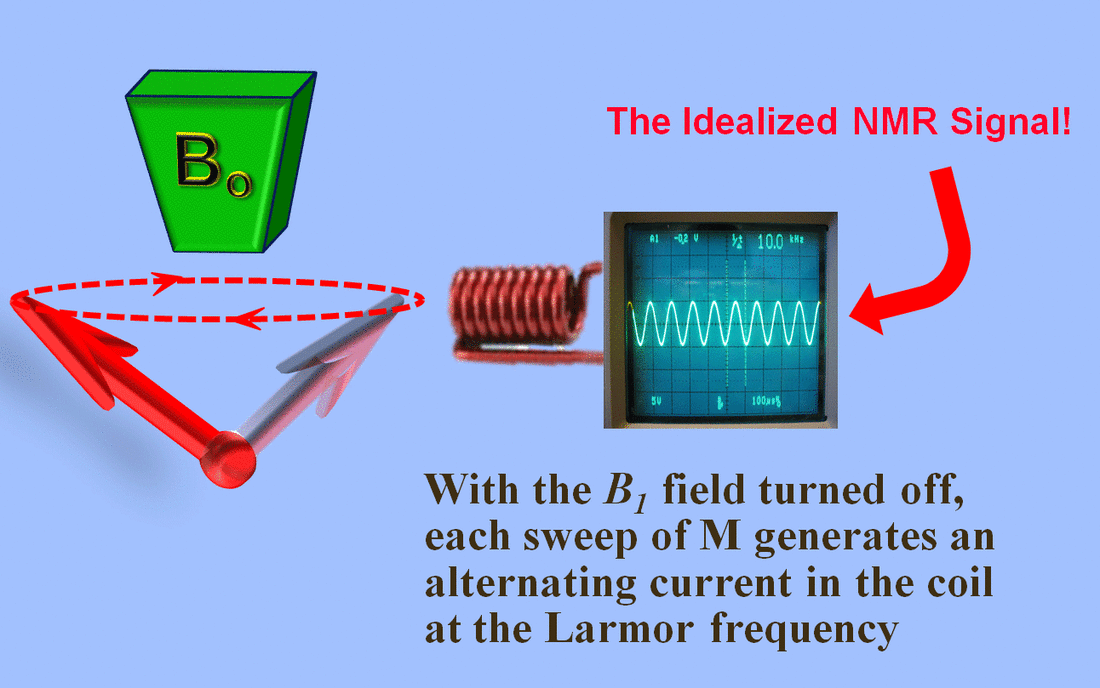
\includegraphics[width=0.3 \linewidth]{figures/FID1.png}
					&
					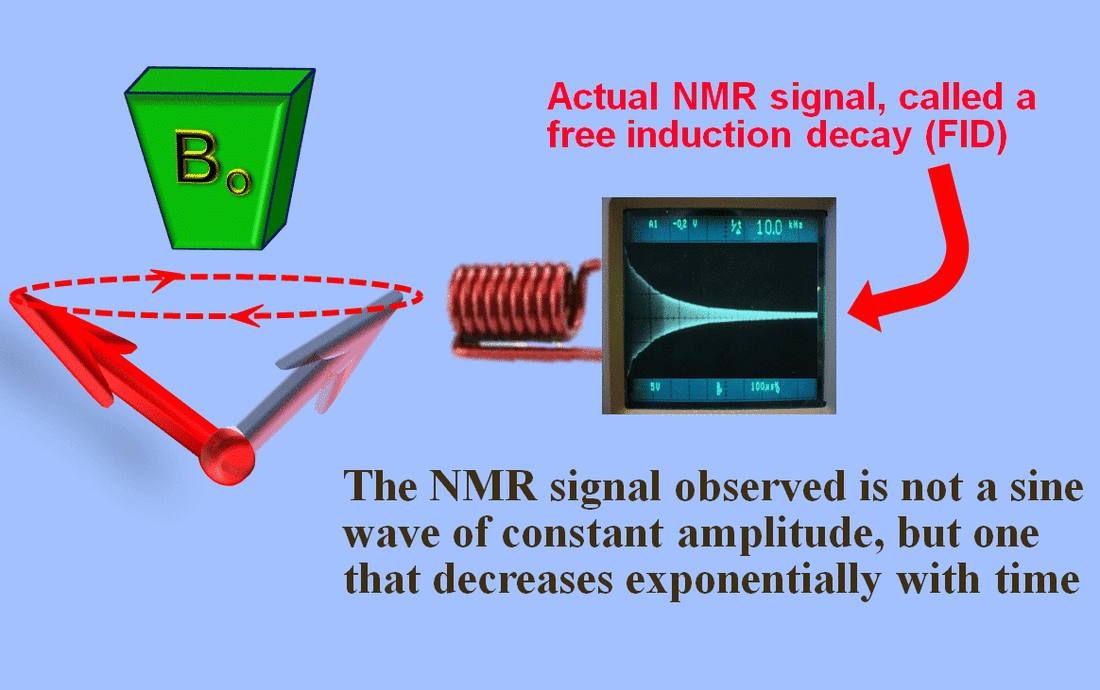
\includegraphics[width=0.3 \linewidth]{figures/FID2.png}
					\\
					
					\mbox{(a) Idealized Signal}
					&
					\mbox{(b) Actual Signal}
				\end{array}$
				\caption{Ideal and Actual Signal \protect \cite{ref:MRI2}}
				\label{fig:fid}
			\end{figure}
		
		\subsection{Fourier Transform}
			A Fourier Transform (TF) is a mathematical transform which decomposes a function in to its constituent frequencies. Also, there are two main algorithm in TF: Discrete Fourier Transform (DFT) and Fast Fourier Transform (FFT). The FFT algorithm derives its efficiency by replacing the computation of one large DFT with that of several smaller DFTs. \cite{ref:FFT1}
	
	\section{Method}
		In this section, the example code will be displayed. However, there are many repetition parts in the program; in this case, only the first part will be shown. 
	
		\subsection{Initializing}
			In this step, the parameters which will be used in entire program will be set, and the raw data are loaded. 
			
			\lstinputlisting[language=matlab, firstline=5, lastline=25]{../FID_recon_and_fitting.m}
	
		\subsection{FID Data Reconstruction}
			In this step, the k-space is re-constructed from the raw data by the Inverse Fourier Transform algorithm. Also, the MRI images are derived from the k-space. 
		
			\lstinputlisting[language=matlab, firstline=67, lastline=96]{../FID_recon_and_fitting.m}
		
		\subsection{$T_1$, $T_2$, $T_2^*$ Fitting}
			In this step, $T_1$, $T_2$, $T_2^*$ fitting is performed with the average of signal. The average of signal is calculated by the equation \ref{eq:average}.
			
			\begin{equation}
				\rm{Average} = \frac{\Sigma \ Signal}{\rm{Number \ of \ Signal}}
				\label{eq:average}
			\end{equation}
		
			\lstinputlisting[language=matlab, firstline=270, lastline=289]{../FID_recon_and_fitting.m}
		
		\subsection{$T_1$, $T_2$, $T_2^*$ Mapping}
			$T_1$, $T_2$, $T_2^*$ Mapping is executed on all of the voxels in the images. 
		
			\lstinputlisting[language=matlab, firstline=448, lastline=471]{../FID_recon_and_fitting.m}
		
		\subsection{Analysis $T_1$, $T_2$, $T_2^*$  by Age}
	
	\section{Results}
		\subsection{FID Data Reconstruction}
			\subsubsection{RARE-VTR FID Image}
				
				\begin{figure}[htbp]
					\centering
					$\begin{array}{ccc}
						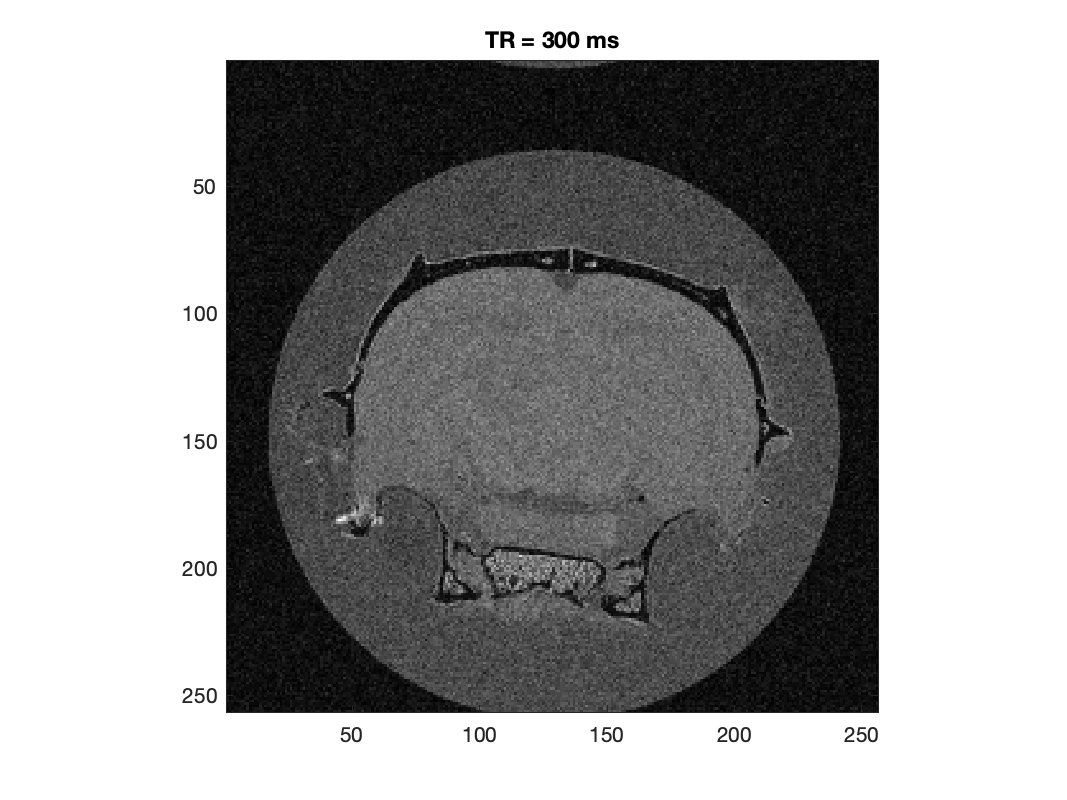
\includegraphics[width=0.3 \linewidth]{figures/VTR_4month/VTR_1.png}
						&
						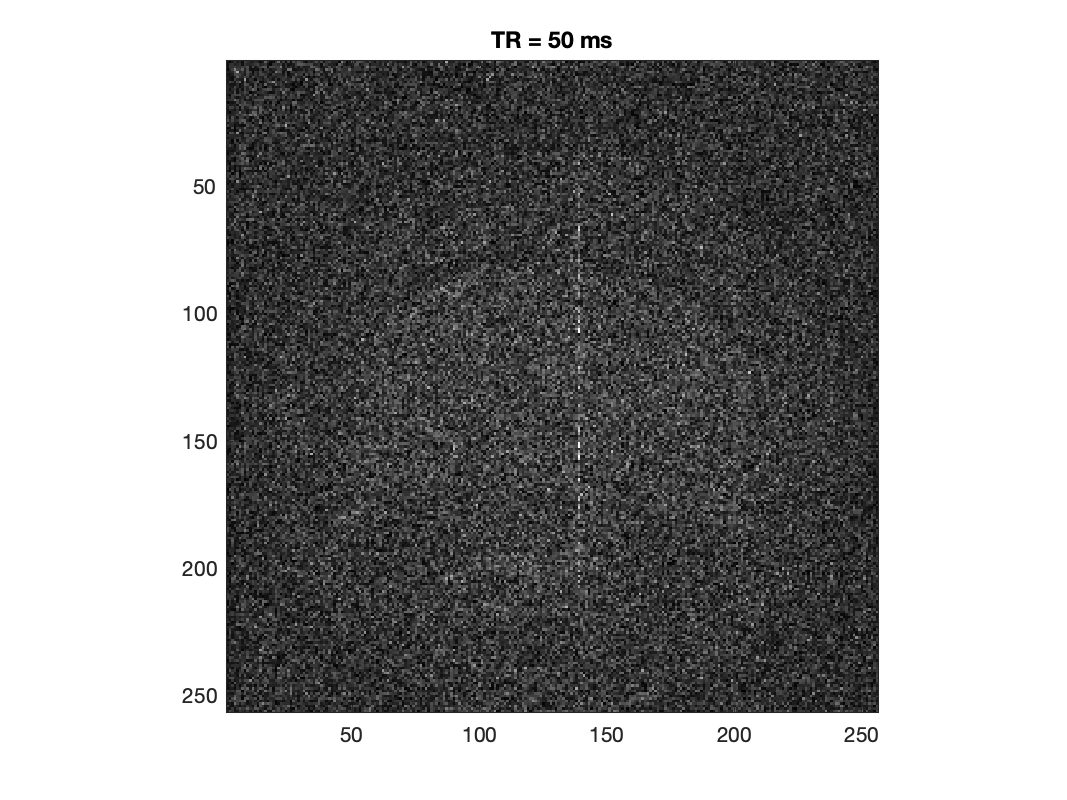
\includegraphics[width=0.3 \linewidth]{figures/VTR_4month/VTR_2.png}
						&
						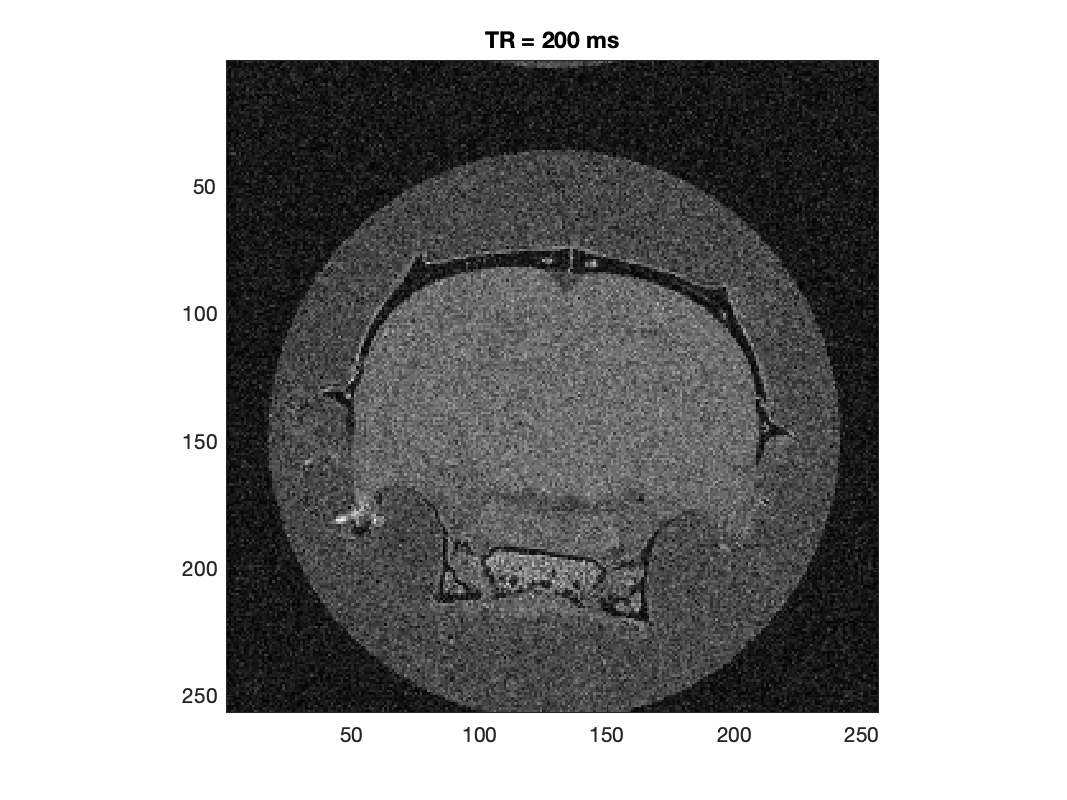
\includegraphics[width=0.3 \linewidth]{figures/VTR_4month/VTR_3.png}
						\\
						\mbox{(1)} & \mbox{(2)} & \mbox{(3)} \\
						
						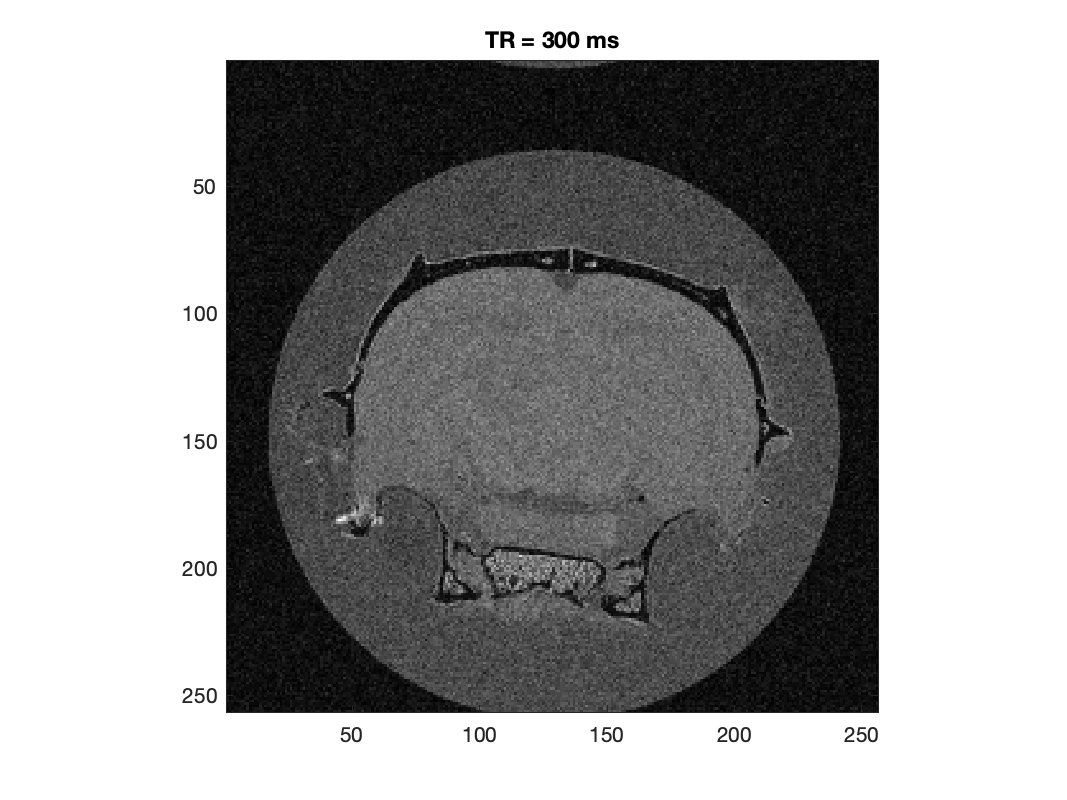
\includegraphics[width=0.3 \linewidth]{figures/VTR_4month/VTR_4.png}
						&
						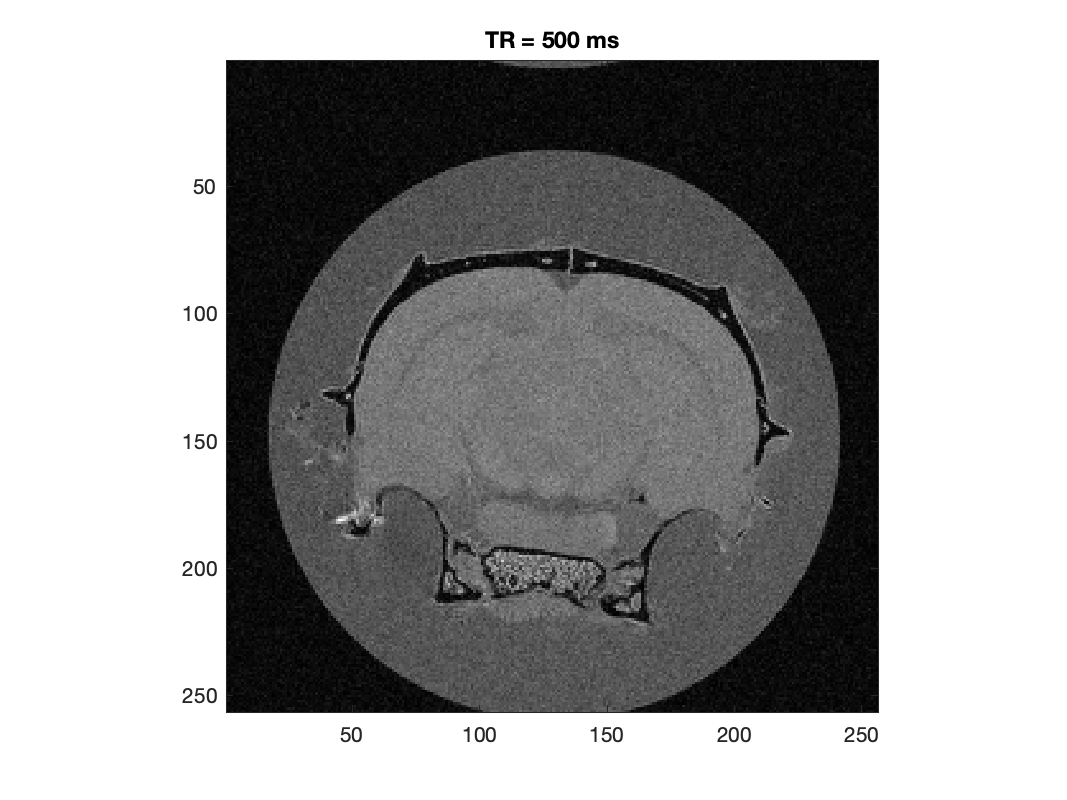
\includegraphics[width=0.3 \linewidth]{figures/VTR_4month/VTR_5.png}
						&
						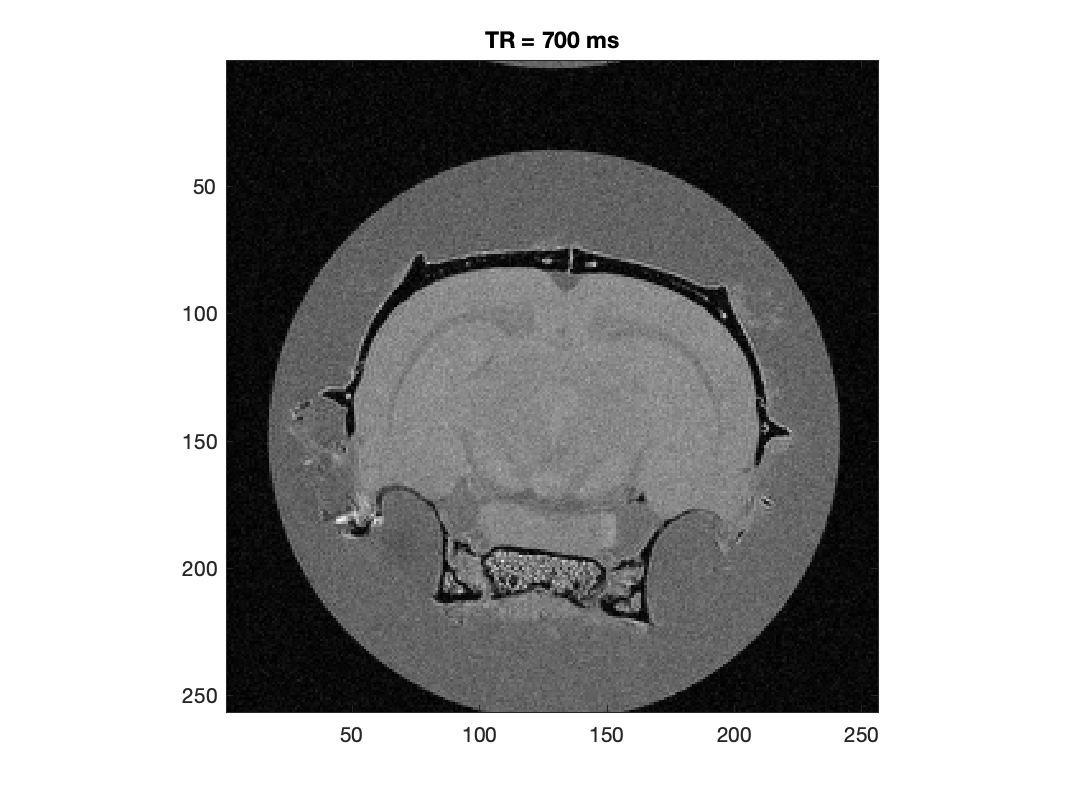
\includegraphics[width=0.3 \linewidth]{figures/VTR_4month/VTR_6.png}
						\\
						\mbox{(4)} & \mbox{(5)} & \mbox{(6)} \\
						
						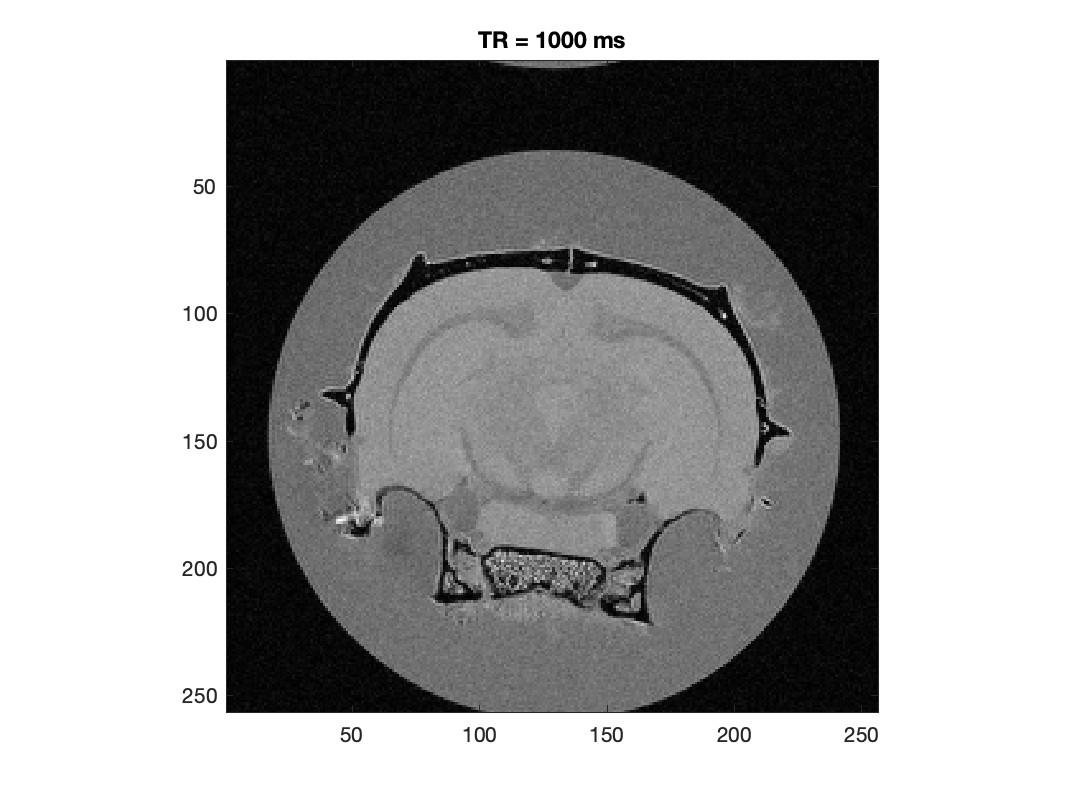
\includegraphics[width=0.3 \linewidth]{figures/VTR_4month/VTR_7.png}
						&
						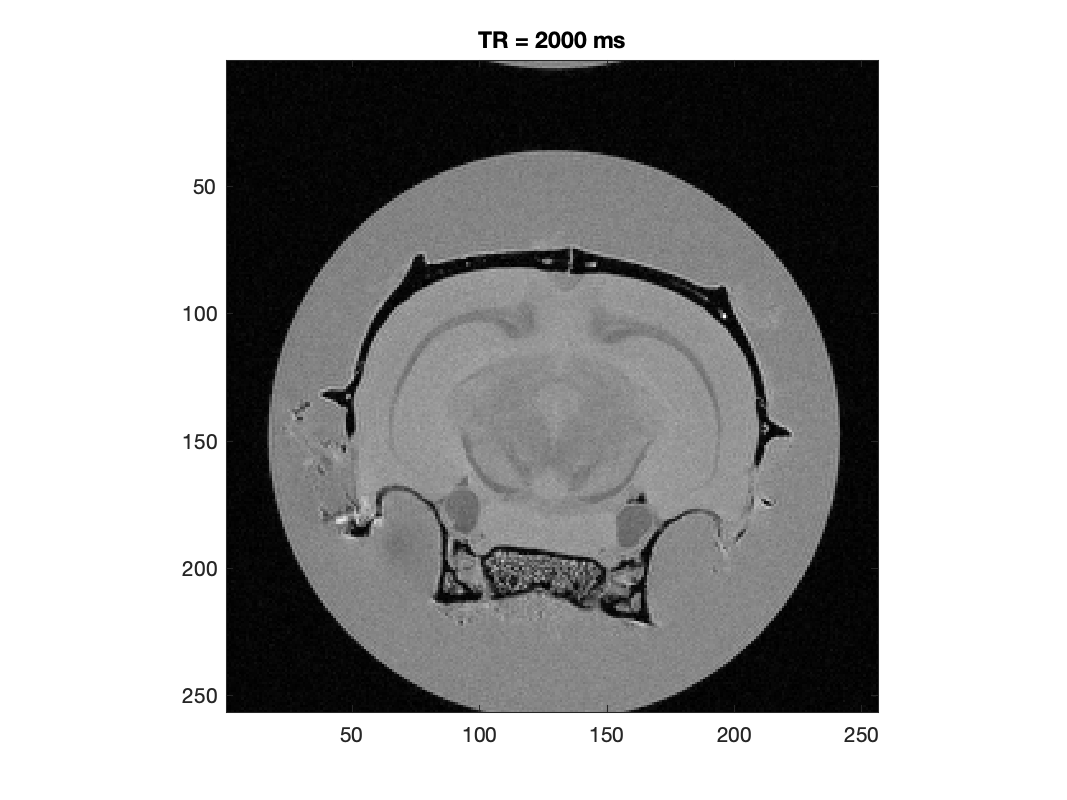
\includegraphics[width=0.3 \linewidth]{figures/VTR_4month/VTR_8.png}
						&
						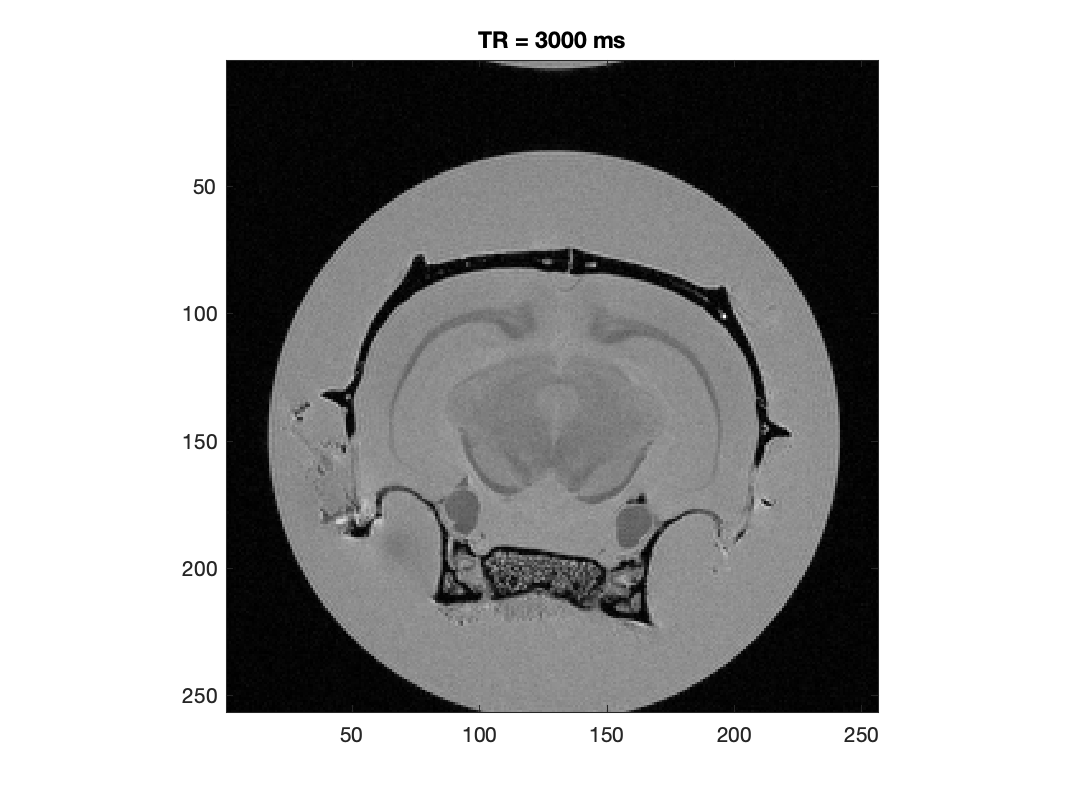
\includegraphics[width=0.3 \linewidth]{figures/VTR_4month/VTR_9.png}
						\\
						\mbox{(7)} & \mbox{(8)} & \mbox{(9)} \\
						
						&
						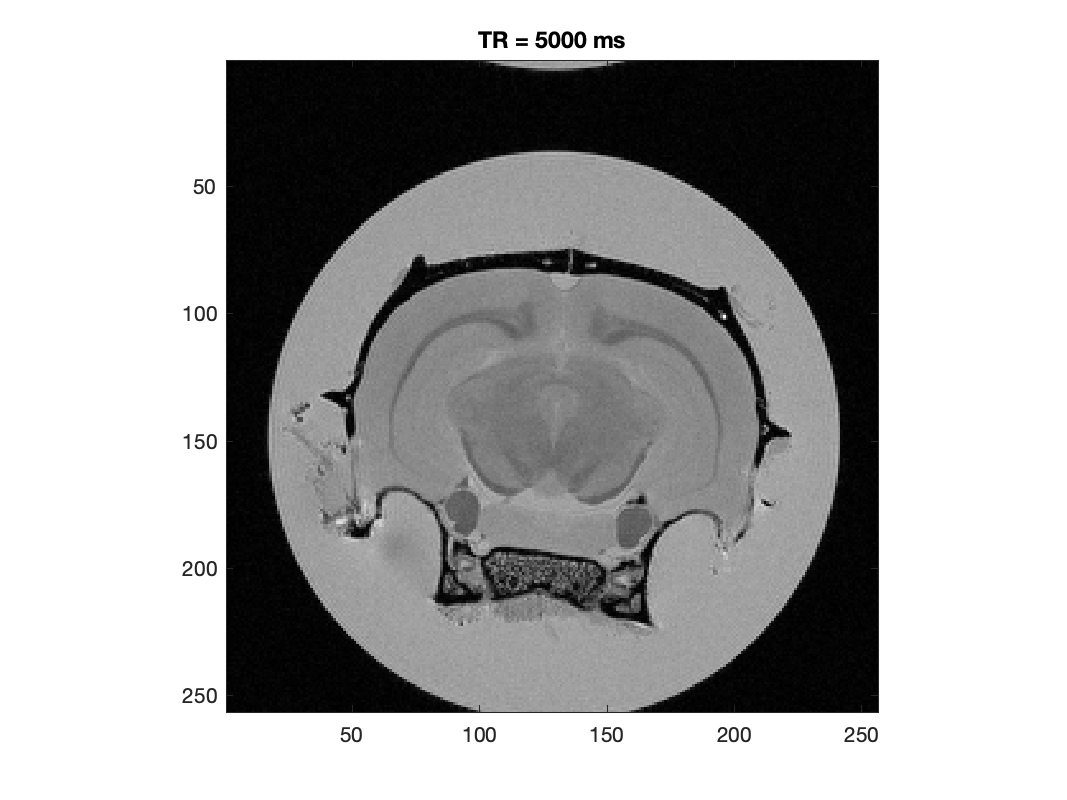
\includegraphics[width=0.3 \linewidth]{figures/VTR_4month/VTR_10.png}
						&
						\\
						& \mbox{(10)} & \\
					\end{array}$
					\caption{RARE-VTR FID Images in 4 month}
					\label{fig:vtr_4month_image}
				\end{figure}
			
			
		
		\subsection{$T_1$, $T_2$, $T_2^*$ Fitting}
		
		\subsection{$T_1$, $T_2$, $T_2^*$ Mapping}
		
		\subsection{Analysis $T_1$, $T_2$, $T_2^*$  by Age}
	
	\section{Discussion}
	
	\addcontentsline{toc}{section}{References}
	\bibliographystyle{apacite}
	\bibliography{reference}
\end{document}